\chapter{Parser Top-Down}
Un \textbf{parser Top-Down} è un tipo di analizzatore sintattico per analizzare strutture gerarchiche, come le frasi di una lingua o la struttura di un codice. \red{Funziona esplorando e costruendo l'albero sintattico partendo dalla radice e procedendo verso le foglie}, quindi "dall'alto verso il basso"

Adesso presentiamo un primo esempio di parser Top-Down \textbf{nondeterministico} che usa implicitamente una pila per gestire le chiamate ricorsive

\section{Parser a discesa ricorsiva}
Data una grammatica libera $G = (NT,T,S,R),\forall A\in NT$ con produzioni:
\[
    A\to X_1^1\dots X^1_{n_1} |\dots|    X_k^1\dots X^k_{n_k}
\]

Definisce la funzione
\begin{algorithm}
    \caption{A()}

    scegli non deterministicamente $h$ tra $1$ e $k$, ovvero una produzione $X_k^h\dots X^h_{n_h}$\;
    \For{$i=1$\KwTo $n_h$}{
        \If{$X_i^h \in NT$}{Nothing()\;}
        \ElseIf{$X_i^h = \text{ simbolo corrente dell'input}$}{
            avanza di un simbolo nell'input\;
        }
        \Else{
            Fail() \tcp*{backtracking! si torna alla riga 2 e si sceglie un'altra produzione}
            \Return\;
        }
    }
\end{algorithm}

Si comincia invocando la funzione per il simbolo iniziale $S$

\esempio{
    Sia $G$ la grammatica:
    \[
        S\to ac|aSb
    \]
    Col linguaggio:
    \[
        L = \{a^{n+1}cb^n|n\geq 0\}    
    \]
    e sia $aacb$ un input.
    Si ha
    \begin{center}
        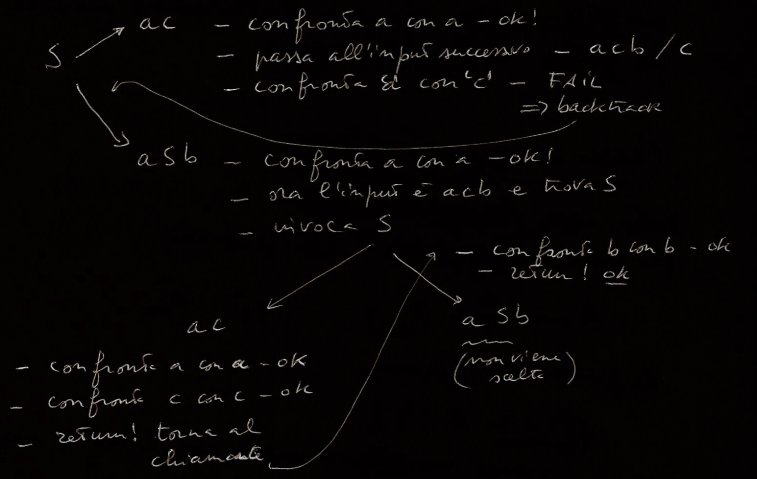
\includegraphics[width=10cm]{top-down_discesa_esempio.png}
    \end{center}

    \begin{center}
            \begin{tabular}{c c}
            \textbf{input} & \textbf{Stack delle chiamate} \\
            \\
            \underline{a} a c b & S \\
            \phantom{a}  & \underline{a} c \\
            \phantom{a} \underline{a} c b & c \textit{fail} \\
            \\
            \underline{a} a c b & S \\
            \phantom{a} & \underline{a} S b \\
            \phantom{a} \underline{a} c b & S b \\
            \phantom{a} & \underline{a} c b \\
            \phantom{a} \underline{c} b & \underline{c} b \\
            \underline{b} & b \\
            & \underline{ok} \\
            \end{tabular}
    \end{center}
}
Tuttavia il parser a discesa ricorsiva è \red{parecchio inefficiente a causa della sua natura nondeterminista}, vi è infatti la necessita nel peggiore dei casi di esplorare tutte le alternative

\teorema{
    Sia $w$ la lunghezza della stringa in inout, e sia $b$ il  massimo numero di produzioni per uno stesso nonterminale, allora la complessità computazionale di un parser a discesa riscorsiva nel caso peggiore è:
    \[
        O(b^{|w|})    
    \]
}

Per ovviare ovviare a questo problema di infecenza dobbiamo guidare la scelta della produzione per creare un parser top-down deterministico. Per farlo occorrono delle fuzioni ausiliarie

\section{Parser predittivo}
Il \textbf{parser predittivo} è un tipo parser deterministico (sotto alcune specifiche condizione che si vedranno più avanti), molto più efficiente in quanto non ha il backtracking, tuttavia per definirlo occorre prima definire delle funzioni ausiliarie
\subsection{First}
\dfn{First}{
    Data una grammatica libera $G \text{ e }\alpha\in(T\cup NT)^*$, di definisce \textbf{First($\alpha$)} come l'insieme dei terminali che possono stare in prima posizione in una stringa che si deriva da $\alpha$ 
    \begin{itemize}
        \item per $a \in T, a \in First(\alpha) \iff \alpha \implies^* a\beta \text{ per }\beta\in(T\cup NT)^*$
        \item inoltre $(\alpha \implies^*\epsilon)\implies \epsilon \in First(\alpha)$
    \end{itemize}
}
\osservazione{
    Sia la grammatica
    \[
        A \to \alpha_1 | \alpha_2       
        \]
        Se $First(\alpha_1)\cap First(\alpha_2) = \emptyset$ la scelta della produzione è deterministica
        }
Qui vi è riportato un esempietto:
\esempio{
    \[
        A\to aB|bC       
    \]
    Si ha che:
    \begin{array}{l}
        First(aB)= \{a\} \\
        First(bC) = \{b\} 
    \end{array}
    Pertanto abbiamo del determinismo con un solo carattere in lettura
}
\subsubsection{algoritmo per calcolare il first}
\begin{algorithm}[H]
    \SetAlgoNlRelativeSize{-1}
    \SetNlSty{textbf}{}{}
    \caption{First()}
    \KwIn{Una grammatica credo}
    \KwOut{bho}
    
        \For{$x\in T$}{
            $First(x)\gets \{x\}$\tcp*{un terminale è il primo elemento di se stesso}
        }
        \For{$X\in NT$}{
            $First(X)\gets \emptyset$\tcp*{per ogni x non terminale si inizializza il suo first a "0"}
        }
        \While{
            almeno un $First(X)$ può essere modificato in una iterazione\
        }{
            \ForEach{$x\to Y_1,\dots,Y_k$}{
                \ForEach{$i=1$\KwTo $k$}{
                    \tcp{se ciascuno di questi simboli $y_1,\dots,Y_{i-1}$ può derivare la stringa vuota $\epsilon$}
                    \If{$Y_1,\dots,Y_{i-1}\in N(G)$ }{
                        $First(X)\gets First(X)\cup (First(Y_i)\backslash\{\epsilon\})$\tcp*{allora è possibile aggiungere gli elementi di $FIRST(Y_i)$ a $FIRST(X)$ per la produzione y_1,\dots,y_k}
                    }
                    \tcp{Se invece uno dei simboli da $Y_1$ a $Y_{i-1}$ non è annullabile, si interrompe la ricerca per quella produzione, perché non possiamo "saltare" i simboli non annullabili per arrivare a Y_i}
                }
            }
        }
        \ForEach{
            $X\in N(G)$
        }{
            $First(X) = First(X)\cup\{\epsilon\}$\;
        }
\end{algorithm}

In generale per una stringa $\alpha$ si ha che:
\begin{itemize}
    \item Se \( \alpha = \varepsilon \), allora \( FIRST(\alpha) = \{\varepsilon\} \).
    \item Se \( \alpha = X \beta \) e \( X \notin N(G) \), allora \( FIRST(X \beta) = FIRST(X) \).
    \item Se \( \alpha = X \beta \) e \( X \in N(G) \), allora $FIRST(X \beta) = (FIRST(X) \setminus \{\varepsilon\}) \cup FIRST(\beta)$
\end{itemize}

In pratica se 
\[
    A\to \alpha_1 | \dots | \alpha_k    
\]
si ha che
\[
    First(A) = First (\alpha_1)\cup\dots\cup First(\alpha_k)   
\]

\esempio{
    Si ossrvi la seguente grammatica:
    \[
        \begin{array}{l}
            S\to Ab|c\\
            A\to aA|\epsilon
        \end{array}       
    \]

    \begin{align*}
        FIRST(S) &= FIRST(Ab) \cup FIRST(c) \\
                 &= (FIRST(A) \setminus \{\epsilon\}) \cup FIRST(b) \cup \{\epsilon\} \\
                 &= \{a\} \cup \{b\} \cup \{c\} = \{a, b, c\}
    \end{align*}
    
    \begin{align*}
        FIRST(A) &= FIRST(aA) \cup FIRST(\epsilon) \\
                 &= \{a\} \cup \{\epsilon\} = \{a, \epsilon\}
    \end{align*}
}
\subsection{Follow}
\dfn{Follow}{
    Data una grammatica libera \( G \) e \( A \in NT \), definiamo che \( Follow(A) \) è l'insieme dei terminali che possono comparire immediatamente a destra di \( A \) in una forma sentenziale.

    \begin{itemize}
        \item Per ogni \( a \in T \), \( a \in Follow(A) \) se \( S \Rightarrow^* \alpha A a \beta \) per qualche \( \alpha \) e \( \beta \in (T \cup NT)^* \).
        
        \item \( \$ \in Follow(A) \) se \( S \Rightarrow^* \alpha A \) (Poiché \( S \Rightarrow^* S \), allora \( \$ \in Follow(S) \) !)
    \end{itemize}
}
Riporto qui un esempio 
\esempio{
    \begin{align*}
        S &\rightarrow A b \mid c \\
        A &\rightarrow a A \mid \varepsilon
    \end{align*}
    
    \[
    Follow(S) = \{\$\} \quad Follow(A) = \{b\}
    \]
    
    \begin{itemize}
        \item \( S \Rightarrow^* S \)
        \item \( S \Rightarrow^* Ab \)
    \end{itemize}    
}
\subsubsection{algoritmo per calcolare il Follow}
\begin{algorithm}[H]
    \SetAlgoNlRelativeSize{-1}
    \SetNlSty{textbf}{}{}
    \caption{Follow()}
    \KwIn{Una grammatica credo}
    \KwOut{bho}
    
        \ForEach{$X\in NT$}{
            $First(X)\gets \emptyset$\tcp*{per ogni X non terminale si inizializza il suo first a "0"}
        }
        $Follow(S)\gets \{\$\}$\;
        \While{
            almeno un $Follow(X)$ può essere modificato in una iterazione
        }
        {
            \ForEach{$X\to\alpha Y\beta$}{
                $Follow(Y)\gets Follow(Y)\cup(First(\beta)\backslash \{\epsilon\})$\;
            }
            \ForEach{$X\to\alpha Y$}{
                \ForEach{$X\to \alpha \beta, \epsilon\in First(\beta)$}{
                    $Follow(Y)\gets Folloe
                    (Y)\cup Follow(X)$\;
                }
            }
        }
\end{algorithm}
in pratica, occorre cercare tutte le produzioni in cui $Y\in NT$ appare e, per ognuna di esse, applicare la 1 o la 2 sopra
\esempio{
    \begin{center}
        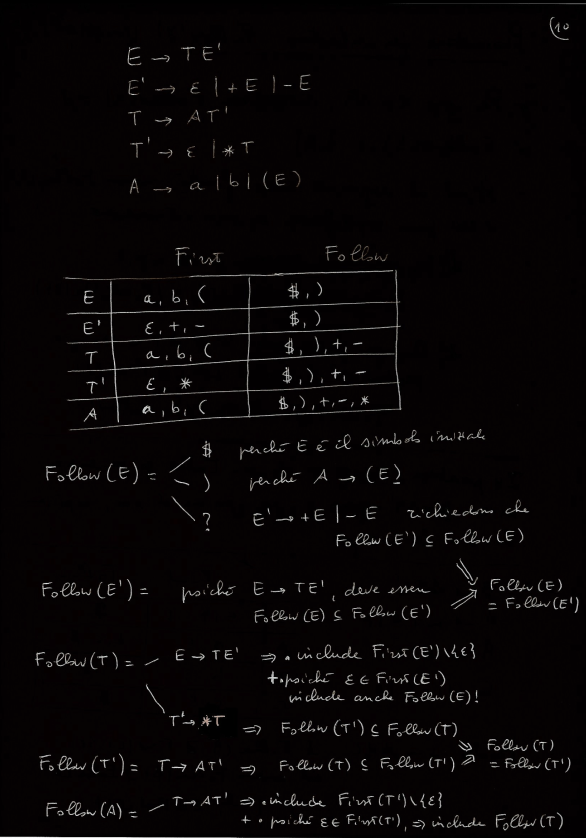
\includegraphics[width=10cm]{esempio_follow.png}
    \end{center}
}
Adesso che abbiamo introdotto i le procedure First e Follow occorre fare un passo in più per definire i parser

\subsection{Parser per linguaggi $LL(1)$}
\subsubsection{tabella di parsing LL(1)}
La tabella di parsing $LL(1)$ è una struttura di dati usata nei parser sintattici molto utili per risolvere il non determinismo. Questi parser leggono l'input da sinistra a destra (da qui il primo "L" di "LL"), costruendo una derivazione sinistra, o leftmost (da qui il secondo "L") e usano un solo simbolo di lookahead (da cui il "(1)").

Questa tabella è formata da una \textbf{matrice bidimensionale $M$} che è formata da:
\begin{itemize}
    \item \textbf{righe}: non-terminali
    \item \textbf{colonne}: terminali (incluso \$)
    \item \textbf{casella} $(A, a)$: $M[A, a]$ contiene le produzioni che possono essere scelte dal parser mentre tenta di espandere $A$ e l'input corrente è $a$.
\end{itemize}

Se ogni casella contiene \red{al più una produzione}, allora il parser è \red{deterministico}!


Per riempire la tabella occorre procedere in questo modo:

Per ogni produzione $A \rightarrow \alpha$:
\begin{enumerate}
    \item per ogni $a \in T$ e $a \in \text{First}(\alpha)$, inserisci $A \rightarrow \alpha$ nella casella $M[A, a]$
    \item se $\varepsilon \in \text{First}(\alpha)$, inserisci $A \rightarrow \alpha$ in tutte le caselle $M[A, x]$ per $x \in \text{Follow}(A)$ (x può essere \$)
\end{enumerate}

Ogni casella vuota, dopo aver elaborato tutte le produzioni, è un errore (cioè la funzione ricorsiva chiama `fail')

\subsubsection{grammatica $LL(1)$}

\dfn{grammatica $LL(1)$}{
    Una grammatica si definisce $LL(1)$ sse ogni casella della tabella di parsing $LL(1)$ contirne al più una produzione, ovvero non presenta conflitti
}

Si ha che \red{se $G=LL(1)$ allora il parser è predittivo e deterministico}, questo perché il parser ricostruisce l'albero di derivazione per l'input $w$, in modo top-down, predicendo quale produzione usare (tra le molte possibili) guardando il prossimo carattere dell'input

\teorema{
    $G$ è $LL(1)$ sse per ogni coppia di produzioni distinte con la stessa testa 
    \[
        A\to \alpha|\beta       
    \]
    si ha che \begin{enumerate}
        \item $First(\alpha)\cap First(\beta)=\emptyset$
        \item \begin{enumerate}
            \item $(\epsilon\in First(\alpha))\implies (First(\beta)\cap Follow(A) = \emptyset)$
            \item $(\epsilon\in First(\beta))\implies (First(\alpha)\cap Follow(A) = \emptyset)$
        \end{enumerate}
    \end{enumerate}
}
\dimostrazione{
    Se sono soddisfatte le condizione 1 e 2 per ogni coppia di produzioni distinte con medesima testa allora la tabella di parsing $LL(1)$ contiene al più una prodizone in ogni cassella. 
    Ma vale anche viceversa!
}

\subsubsection{Linguaggio $LL(1)$}
\dfn{Linguaggio $LL(1)$}{
    Un linguaggio si definisce $LL(1) \iff \exists G' \text{ grammatica } = LL(1)$ che lo genera 
}
\esempio{
    Sia $G$ la segunete grammatica:
    \[
        \begin{array}{l}
            S\to A|B\\
            A \to ab|cd\\
            B\to ad|cb
        \end{array}       
    \]
    Si può notare che $G$ non è $LL(1)$ dato che $S\to A|B$ e 
    \[
        \begin{array}{l}
            First(A) = \{a,c\}\\
            First(B) = \{a,c\}\\
            First(A)\cap First(B) = \{a,c\}
        \end{array}
    \]
    Dal teorema sopra fornito si può dimostrare che non è $LL(1)$\\
    Tuttavia si può manipolarla per farla diventare $LL(1)$, quindi espando $S$:
    \[
        S\to ab|cd|ad|cb    
    \]
    \[
        \begin{array}{l}
            S\to aT|cT'\\
            T\to b|d\\
            T'\to b|d
        \end{array}    
    \]
    Poi osservo che $T$ e $T'$ sono identici, sia quindi $G'$ la nuova grammatica:
    \[
        \begin{array}{l}
            S\to aT|cT  \\
            T\to b|d
        \end{array}
    \]
    Si può dimostrare che è $LL(1)$, pertanto, per la definizione di linguaggio $LL(1)$ e nonostante $G$ non sia $LL(1)$, si ha che $L(G) =\{ ab,cd,ad,cb\}$ è un linguaggio $LL(1)$ perché $G'$ che lo genera è una grammatica $LL(1)$  
    }

    \teorema{
        Ogni linguaggio regolare è generabile da una grammatica $G$ di classe $LL(1)$
    }
    \dimostrazione{
        Sia $L$ un linguaggio regolare, allora $\exists \text{ DFA }M=(Q,\Sigma , \delta, q_0, F):L=[M]$.

        A partira da $M$ si può costruire una grammatica regolare $G=(NT,T,S,R)$ basata sul seguente automa $M$:
        \begin{itemize}
            \item $NT=\{[q]|q\in Q\}$, cioè un non terminale per ogni stato $q$
            \item $T= \Sigma$ cioè un terminale per ogni simbolo dell'alfabeto
            \item $S=[q_0]$ simbolo iniziale lo stato iniziale
            \item $R$ (insieme delle produzioni) è definito come:
            \begin{itemize}
                \item se $\delta (q,a) = q'$, allora $[q]\to a[q']\in R$
                
                Infatti $\delta (q,a) = q'$ vuol dire che l'automa si trova allo stato $q$ e legge in input $a$ allora arriverà allo stato $q'$, che viene "tradotto" nella grammatica $[q]\to a[q']$ che corrisponde ad una produzione in cui il non terminale $[q]$ produce il terminale $a$ e il non terminale $[q']$, per passare al non terminale $[q']$ occorre, infatti, fare match con $a$
                \item se $q\in F$, allora $[q]\to \epsilon\in R$
            \end{itemize}
        \end{itemize}

        Poi che $M$ è deterministico, \( \forall q \in Q \forall a \in \Sigma \quad \exists! q'. q \xrightarrow{a} q' \), cioè \( [q] \) avrà una sola produzione \( [q] \to a[q'] \) che "inizia" per \( a \) e dato che se \( q \) è finale, allora \( [q] \to \epsilon \) è applicabile solo per i \(\text{Follow}([q]) = \{\$\} \implies \text{ nessun conflitto}\), dato che nessuna produzione genera $\$$, si ha che $G$ è $LL(1)$
    }
    \esempio{
        \begin{center}
            \begin{tikzpicture}[shorten >=1pt,node distance=2cm,on grid,auto] 
               \node[state,initial] (q_0)   {$q_0$}; 
               \node[state,accepting] (q_1) [right=of q_0] {$q_1$}; 
                \path[->] 
                (q_0) edge [loop above] node {a} ()
                      edge [bend left]  node {a} (q_1)
                (q_1) edge [bend left]  node {a} (q_0);
            \end{tikzpicture}
            \end{center}
            Le produzioni corrispondenti sono:
            \[
                \begin{array}{l}
                    [q_0] \to a[q_1]  a[q_0] \\
                    [q_1] \to a[q_0] \mid \epsilon
                    
                \end{array}
            \]
            
            La grammatica \( G \) è \( LL(1) \), perché:
            \[
                \text{First}(a[q_0]) \cap \text{First}(\epsilon) = \emptyset, \quad \text{First}(a[q_1]) \cap \text{First}(\epsilon) = \emptyset
            \]
    }
    
    Riporto qui un esempio di tabella di parsing $LL(1)$:
    \esempio{
        Sia $G$ la seguente grammatica:
        \[
            \begin{array}{l}
                E \to T E' \\
                E' \to \varepsilon \, | \, + T E' \, | \, - T E' \\
                T \to A T' \\
                T' \to \varepsilon \, | \, \ast T \\
                A \to a \, | \, b \, | \, (E)
                
            \end{array}       
    \]
    
    Si può costruire la seguente tabella di First e Follow:
    \[
        \begin{array}{|c|c|c|}
            \hline
            \text{Produzione} & \text{First} & \text{Follow} \\
            \hline
            E & a, b, ( & \$, ) \\
            E' & +, -, \varepsilon & \$, ) \\
            T & a, b, ( & +, -, \$, ) \\
            T' & \ast, \varepsilon & +, -, \$, ) \\
            A & a, b, ( & \ast, +, -, \$, ) \\
            \hline
        \end{array}
        \]
        
        Ed ecco a voi la tabella di parsing:
        \[
            \begin{array}{|c|c|c|c|c|c|c|}
                \hline
                & a & b & ( & + & \ast & \$ \\
                \hline
                E & E \to T E' & E \to T E' & E \to T E' &  &  &  \\
                E' &  &  &  & E' \to + T E' & E' \to - T E' & E' \to \varepsilon \\
                T & T \to A T' & T \to A T' & T \to A T' &  &  &  \\
                T' &  &  &  & T' \to \varepsilon & T' \to \ast T & T' \to \varepsilon \\
                A & A \to a & A \to b & A \to (E) &  &  &  \\
                \hline
            \end{array}
            \]
            
            \begin{center}
                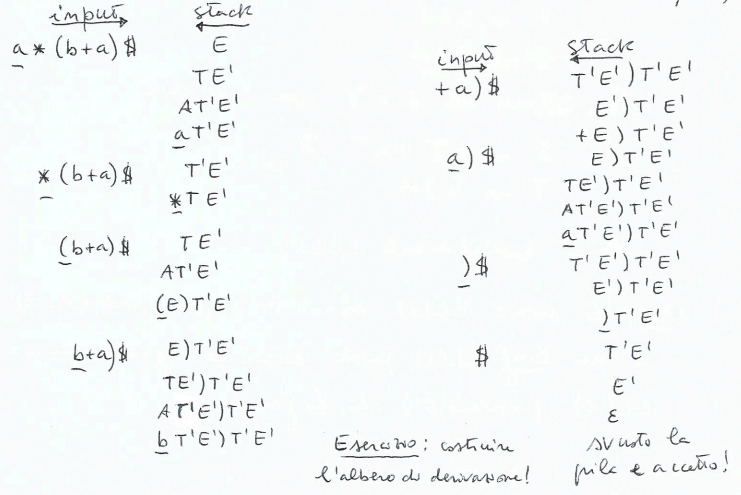
\includegraphics[width=7cm]{Parser_con_pila.png}
            \end{center}   
}

\subsubsection{Algoritmo Per il calcolo di un parser $LL(1)$}

\begin{algorithm}
    \caption{Parser $LL(1)$}
    \KwIn{Stringa $w$}
    \KwOut{Niente}

    $Pila\gets S\$$\tcp*{cima della pila a sinistra}
    $X\gets S$ \tcp*{top della pila}
    \tcp{lettura in input}
    $input \gets w\$$\;
    $i_c = \text{ primo carattere dell'input}$\;
    \tcp{viene eseguito il ciclo While finché la pila non è vuota o l'input non è stato consumato}
    \While{$X\neq \$$}{
        \If{$X$ è un terminale}{
            \tcp{si controlla se $X$ fa "match" con $i_c$}
            \If{$X = i_c$}{
                Pop $X$ dalla pila\tcp*{rimuovo $X$ dalla pila}
                avanza $i_c$ sull'input\;
            }
            \Else{
                Errore()\tcp*{no match}
            }
        }
        \Else{
            \tcp{se nella tabella di Parsing $M$ esiste una regola $X\to Y_1, \dots, Y_n$}
            \If{$M[X,i_c] = X\to Y_1, \dots, Y_n$}{
                Pop $X$ dalla pila\;
                Push $Y_1, \dots, Y_n$ sulla pila \tcp*{mette sulla pila i simboli $Y_1, \dots, Y_n$ con $Y_1$ in cima}
                In output la produzione $X\to Y_1, \dots, Y_n$\; 
            }
            \Else{
                Errore ()\tcp*{se non esiste una regola  in $M[X,i_c]$ si genera un errore, viene definito caso "bianco"} 
            }
            $X\gets$ top della pila\tcp*{Aggiorna $X$ con il nuovo simbolo in cima alla pila}
        }
    }
    \If{$i_c\neq \$$}{
        Errore()\tcp*{pila svuotata ma vi è ancora dell'input da leggere}
    }
\end{algorithm}



Un altro esempio:
\esempio{
    Sia $G$ la seguente grammatica:
    \[
    \begin{aligned}
        S &\to aAB \, | \, bS \\
        A &\to a \\
        B &\to b
    \end{aligned}
    \]
    Che genera il seguente linguaggio
    \[    
        L(G) = L\big(b^*aab\big)
    \]
    Si ha che questa grammatica \(G\) è LL(1), perché:
    \[
        First(aAB) \cap First(bS) = \varnothing, \quad \{a\} \cap \{b\} = \varnothing
    \]

    Si può prosegure con la tabella First e follow:
    \[
        \begin{array}{|c|c|c|}
        \hline
        Simbolo & First & Follow \\
        \hline
        S & a, b& \$ \\
        A & a& b \\
        B & b& \$ \\
        \hline
        \end{array}
    \]
    Da cui si può costruire la seguente tabella di parsing:
    \[
        \begin{array}{|c|c|c|c|}
        \hline
        & a & b & \$ \\
        \hline
        S & S \to aAB & S \to bS &  \\
        A & A \to a &  &  \\
        B &  & B \to b &  \\
        \hline
        \end{array}
    \]
    
    Viene qui descritto il funzionamento del parser con pila con diversi input:
    \begin{center}
        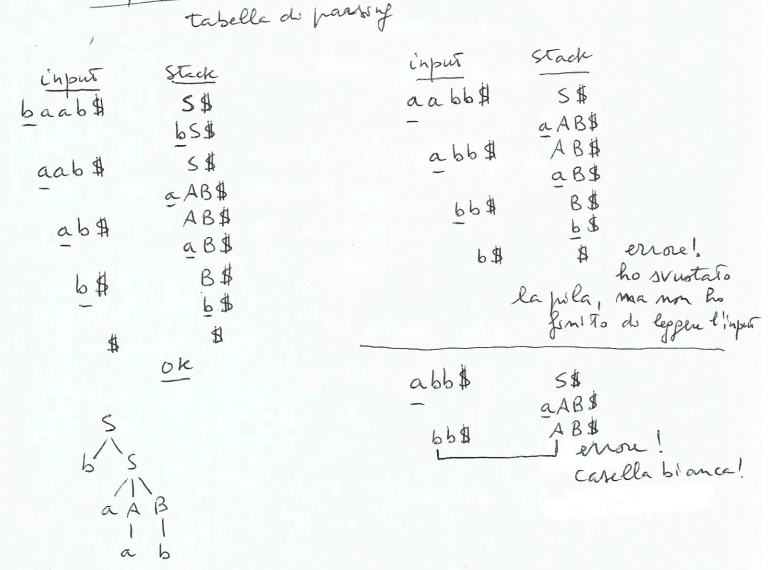
\includegraphics[width=10cm]{parser_pila_2.png}
    \end{center}


}

\subsection{Parser per linguaggi $LL(K)$}
\subsubsection{grammatiche $LL(K)$}
Le grammatiche $LL(k)$ sono "un'estensione" del concetto di grammatiche $LL(1)$, dove il parser ha la capacità di guardare in avanti fino a $k$ simboli per determinare le scelte di parsing

Per questi tipi di grammatica gli insiemi $First \text{ e }Follow$ assumo significati diversi rispetto a alle grammatiche $LL(K)$
\dfn{First $LL(K)$}{
    L'insieme \(First_k(\alpha)\) contiene tutte le stringhe di lunghezza \( k \) o minore derivabili dall'inizio di una produzione con \( \alpha \), in particolare
    $w\in First_k(\alpha) \iff \alpha \implies^{*}w\beta \text{ con } |w|=k,w\in T^{*}, \beta\in (T\cup NT)^* \text{ oppure }  \alpha \Rightarrow^* w  \text{ con } |w| \leq k \text{ e }  w \in T^* $
}
\dfn{Follow $LL(K)$}{
    L'insieme Follow\(_k(A)\) definisce quali stringhe possono apparire immediatamente dopo un simbolo non terminale \( A \) in una derivazione a partire dal simbolo iniziale \( S \). In particolare:
    \( w \in \text{Follow}_k(A) \) se \( S \Rightarrow^* \alpha A w \beta \) con \( |w| = k \), \( w \in T^* \), e \( \alpha, \beta \in (T \cup NT)^* \), oppure, \( S \Rightarrow^* \alpha A w \) con \( |w| \leq k \) e \( w \in T^* \).
}

\subsubsection{Tabella di Parsing $LL(K)$}
\begin{itemize}
    \item \textbf{Righe}: non terminali.
    \item \textbf{Colonne}: $\{ w \in T^* \mid |w| \leq k \}$ (solo quelle necessarie).
\end{itemize}

\noindent Per ogni produzione $A \to \alpha$, la tabella $M[A, w]$ contiene:
\begin{itemize}
    \item $A \to \alpha$, per ogni $w \in \text{First}_k(\alpha)$ ($w \neq \varepsilon$);
    \item $w \in \text{Follow}_k(A)$ se $\varepsilon \in \text{First}_k(\alpha)$.
\end{itemize}

\noindent Ogni entrata/casella contiene al più una produzione. Se non esistono $w_1$ e $w_2$ tali che $w_1$ prefisso di $w_2$ con le due entrate corrispondenti su una riga entrambe riempite, allora $G$ è una grammatica LL(k).

\vspace{1em}
\noindent \textbf{Nota Bene:} 
Le colonne sono tante quante sono le stringhe $w$ che appartengono a $\text{First}_k(\alpha)$ per $A \to \alpha$ o a $\text{Follow}_k(A)$ per $A \to \alpha$. Questo va verificato per tutte le produzioni:
\[
w \in \text{First}_k(\alpha).
\]

\esempio{
    Sia $G$ la seguente grammatica
    \[
        S\to aSb\mid ab\mid c
    \]
    Si ha che $L(G) = \{a^nb^n\mid n\geq 1\}\cup\{a^ncb^n\mid n\geq 0\}$, inoltre:
    \begin{itemize}
        \item $First_2(aSb) =\{aa,ac\}$
        \item $First_2(ab) =\{ab\}$
        \item $First_2(c) = \{c\}$
    \end{itemize}

    Si può dimostrare che $G$ è $LL(2)$ dato che:
    \begin{itemize}
        \item $First_2(aSb)\cap First_2(ab)=\varnothing$
        \item $First_2(aSb)\cap First_2(ab)=\varnothing$
        \item $First_2(aSb)\cap First_2(ab)=\varnothing$
    \end{itemize}
    Da cui si può ricavare la tabella di parsing:
    \[
        \begin{array}{|c|c|c|c|c|}
        \hline
        Simbolo & aa & ab & ac & c \\
        \hline
        S & S \to aSb& S\to ab&S\to aSb & S\to c
        \hline
        \end{array}
    \]

}
        
\teorema{
    \begin{itemize}
        \item Una grammatica ricorsiva sinistra non è $LL(K)$ per nessun $K$
        \item Una grammatica ambigua non è $LL(K)$
        \item Se $G$ è $LL(K)$ per qualche $k$, allora $G$ non è ambigua 
        \item Se $G$ è $LL(K)$, allora $L(G)$ è libero deterministico
        \item esiste $L$ libero deterministico tale che non esiste G di classe $LL(K)$ per nessun $K$, tale che $L=L(G)$
    \end{itemize}
}


Viene qui riportato il funzionamento del parser con pila:
\subsubsection{Linguaggio $LL(K)$}

\dfn{Linguaggio $LL(K)$}{
    un linguaggio $L$ è di classe $LL(K)$ se $G$ di classe $LL(K)$ tale che $L=L(G)$
}

\teorema{
    $\forall k\geq 0$, la classe dei linguaggi $LL(K)$ contiene strettamente la classe dei linguaggi $LL(K)$
}
\osservazione{
    $\forall k\geq 0,$ la classe dei linguaggi $LL(K+1)$ contiene strettamente la classe dei linguaggi $LL(K)$
    \begin{center}
        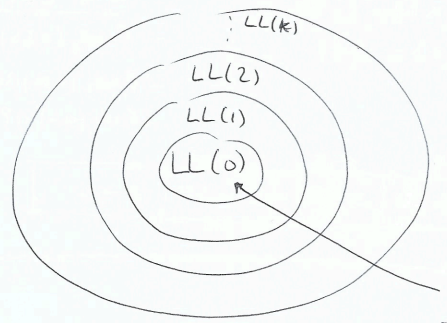
\includegraphics[width=10cm]{gerarchia_dei_linguaggi.png}
    \end{center}
    Si ha che: $(\forall A \in NT, \quad \exists! \alpha \in (T \cup NT)^*, \quad A \to \alpha \implies G \text{ è } LL(0))\implies L(G) = \{w\}$ ovvero una sola parola al massimo
}

\red{Nella pratica tuttavia si usano solo $LL(1)$}, spesso la si può manipolare trasformandola in $LL(1)$

\esempio{
    \[
        \begin{array}
            S\to Asb!ab!c\\
        \end{array}       
        
    \]
    $G$ è un $LL(2)$ ma non $LL(1)$
    Si fattorizza
    \begin{array}{l}
        S\to aT|c\\
        T\to Sb|b
    \end{array}
    Ottenuta fattorizzando $G$ è $LL(1)$ infatti:
    \begin{itemize}
        \item $First(aT)\cap First(c)=\varnothing$
        \item $First(Sb)\cap First(b)=\varnothing$
    \end{itemize}
    Si ha che $L = \{a^n b^n\mid n\geq 1\}\cup \{a^ncb^n\mid n\geq 0\}$ è un linguaggio di classe $LL(1)$ perché $G'$ è $LL(1)$
}
\subsubsection{Casi speciali}
Sia 
\[
    L= \{a^i b^j | i\geq j\} \text{ è libero deterministico}    
\]
Ma non è $LL(K)$ per nessun $K$!

Adesso, mostriamo una grammatica per $L$ e dimostriamo che non è LL(K) per nessun $K$.
Sia $G$ la seguente grammatica:
\[
    \begin{array}{l}
        S\to aS|B\\
        B\to aBb|\epsilon    
    \end{array}
\]

\begin{center}
    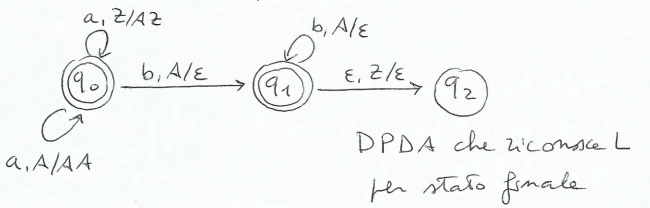
\includegraphics[width=10cm]{l_libero_deterministico_non_LL(K).png}
\end{center}

Sia $G$ una grammatica libero per $L$
\[
    S\to aS\mid B \\
    B\to aBb \mid \epsilon    
\]
e poniamo $L=L(G)$

%! NON HO CAPITO CAZZO

Per scegliere tra $S\to aS$ e $S\to B$ dovrei leggere fino in fondo l'input per sapere quante $b$ in meno di $a$ ci sono nella stringa! Allora $G$ non può essere $LL(k)$ per nessun $k$. Infatti quanto possa essere grande il $K$ posso trovare una stringa più lunga che richiede di leggere più di $k$ simboli di lookahead

Non è tuttavia possibile alcuna $G'$ e $k$ tali che
\[
    L(G') = L \text{ e }G'\in L(K)    
\]
La dimostrazione non verrà illustrata 
